\documentclass[fleqn,10pt]{olplainarticle}
\usepackage{csquotes} % For biblatex formatting
\addbibresource{bibliography.bib} % Bibliography file
\graphicspath{ {./images/} } % Image path

% Use option lineno for line numbers 

\title{Data Science Hazards (TBC)}

\author[1]{First Author}
\author[2]{Second Author}
\affil[1]{Address of first author}
\affil[2]{Address of second author}

\keywords{Keyword1, Keyword2, Keyword3}

\begin{abstract}
An opinion piece about embedding responsibility for worst case scenario impacts of data science research.
\end{abstract}

\begin{document}

\flushbottom
\maketitle
\thispagestyle{empty}

\section*{Introduction}

- Data science needs ethical audit, and like all audits, it should be done by someone qualified and without skin in the game.
  - Data science work has a lot of impact now. It requires a true *ethics* review (not just a legal one). And it requires it early in the process BEFORE it is applied and harms people.
  - Data scientists are not equipped to do this work. They are not trained to do this work. They do not feel qualified to do this work. Incentives in research and industry mean that they are well-practised at making cases for the good aspects of their work (efficiency, accuracy), but have little experience in considering the worst case scenarios of this work.
  - Social science and humanities researchers are well-practised at considering the societal impact of things, they are good at imagining digital futures. Their work tends to be segregated from data science work. It is not embedded in the process. It is published separately. 
- The pipeline of research to deployment is long and winding: we need to make it very easy for people to notice the potential impacts. So we suggest colourful labels applied at every stage, to help pass responsibility between different stakeholders like a baton.
  - People who are buying data science solutions (representatives from for example local authorities, police, private companies) are likely to be talking to data scientists, or more likely sales representatives, or other representatives from a data science company, one or more degrees removed from the technology. Very unlikely to be shown potential negative impacts.
  - So much of research is so abstract, so far removed from reality and any form of "impact" that it can seem pointless to consider it. There are many stages in the process, many minor technical achievements that stack on top of one another, and could be used for positive or negative uses. AI has many positive uses. It has many negative uses. At each stage, new doors open as to what is possible. At each stage, we need to avoid Jurassic Park (consider if it's good/useful, not just if it's possible). We need to make it easy for the people who are putting this into production to take responsibility for what it is that they are putting into production. 
  
 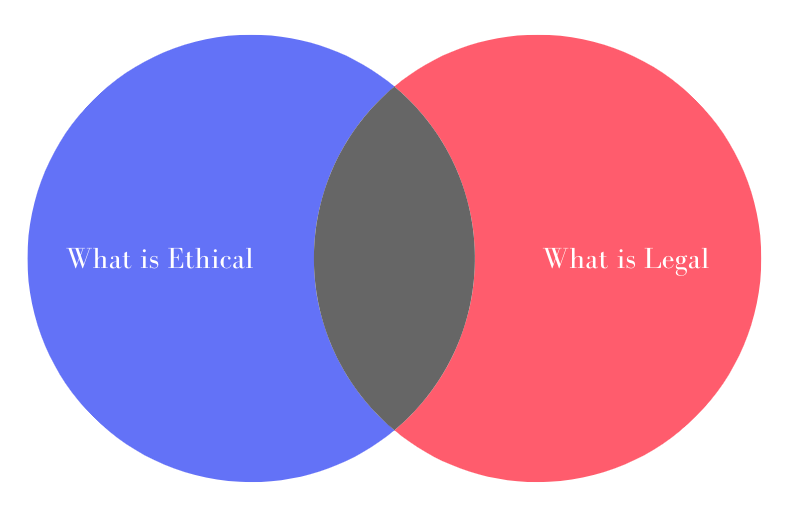
\includegraphics[scale=0.35]{ethical-legal.png}

 
\section*{The power of worst case scenarios}
  
- The power of worst case scenarios is that we don't need to be able to see the future. We're not arguing about what will happen, we are just making sure that you know that it could happen, so if you are using this technology, it's your responsibility to ensure that it does not.
  - We suggest considering worst case scenarios. This doesn't mean that the research shouldn't be done, just that negative impacts must be considered (if ALL the impacts are negative, then yes don't do it).  
  
- An existing example of this is 'Consequence Scanning' (developed by DotEveryone https://doteveryone.org.uk/), which is part of the agile methodology, focussed on software development. 
- What we are describing here is a methodology for incorporating something a la consequence scanning into academic research, rather than just at the stage of developing a product. Consequence scanning is designed for agile teams, and many researchers don't work in those types of environments. We're also suggesting that wider expert perspectives (i.e. from politics/sociology) should be invited at the beginning.

- Not a substitute for co-designing research (involvement of the people who will be affected by it).

\section{Hazard labels}
- We present one way of doing this: putting colourful labels on the research itself. Like chemical hazards. 
  - It is designed as an interdisciplinary consideration. Just as data scientists work with other specialists (software engineers, library/data management professionals, lawyers), we want to normalise this type of interaction.
- The labels themselves.
  - There is a finite number of them. This is to make the task of auditing easier (like chemicals, like ethical review tick boxes) and more importantly, the task of understanding the audit easier.
  - This is not a substitute for a detailed consideration. It is in addition to the existing work that is happening.
  - We got help from social scientists to consider what types of hazards have a good coverage of negative impacts, e.g. environmental, hazardous to human health, reinforces inequity, harmful to the implementer.
  - We got an artist to design them.
- How it works
  - Test out by consulting social scientists (Bristol Digital Futures Institute? Brigstow Institute?), who are then acknowledged on the data science papers that they consult on, similar to statistical consulting (a la Ask-JGI) for seedcorn funding. (To be clear, I am imagining they would be authors on the data hazards paper).
  - Must show the hazard label when you present (condition of funding) and when you publish. We provide a statement to help people interpret it.
  - If you want to do this, then this is how to join in as a social scientist/philosopher/historian, and this is how to do this as a data scientist (maybe we could have a properly ethical review panel set up).

\section*{Arguments against Hazard Labels}

- Perverse incentive to do this because it will be difficult to fund work that has made the potential negative outcomes clear.
  - Funding applications that build on "hazardous" research should consider whether the extra research gets us closer or further from worst case scenarios.
  - It's a fair point, though! Hazard label to our work: could reduce funding of ethical research.
  
- Give people ideas for evil schemes. Makes sure that we can do something to prevent it rather than being caught out when they surreptitiously think it up.

\section*{Acknowledgments}

Thank you to all the people who read the draft for us. 

\printbibliography

\end{document}